\documentclass[12pt]{paper}

\usepackage{Schwieg}
\usepackage[margin=.75in]{geometry}
\usepackage{tikz}

\title{Price Theory 1 - Problem Set 2 - Question 1}
\author{Timothy Schwieg \and Samuel Barker \and Rafeh Qureshi \and Ana Vasilj
 \and Daniel Noriega}

\begin{document}

\maketitle

\section*{Setup}
Consider a world with three agents: Consumers, Firms producing food,
and firms producing cars. We assume the standard quasi-concave
preferences etc.

Technology in this world is linear, and the only factor of production
is labor. Assume that food firms produce $m$ units of food per unit
labor and that car firms produce $c$ units of cars per unit
labor. Individuals are also able to produce food at the same rate of
$m$ units of a food per unit time.

\subsection*{Consumers}

Consumers are able to produce food at home, producing $m$ units of
food per unit time. They are able to work at either car or food firms
freely and receive wages $w_v, w_f$ respectively. However they view
food produced in the market and from their house as perfect
substitutes.

The question they face is:
\begin{align*}
  \max_{\ell,f_H,f_m,v} \quad &U( f_H + f_m, v)\\
  \text{s.t. } &\ell \in [0,1]\\
                       &f_H = (1-\ell)m\\
  &\ell \overline{w} = p_v v + p_f f_m
\end{align*}

Where $\ell$ is the amount of time they spend working, $f_H$ is food
produced at home, $f_m$ is food bought at market, and $v$ are the
vehicles bought at market. $\overline{w}$ is the maximum of the two
wages earned by working for the food and vehicle firms.

Rearranging the constraints and using $\ell = 1 - \frac{f_H}{m}$. 
\begin{align*}
  \max_{\ell,f_H,f_m,v} \quad &U( f_H + f_m, v)\\
  \overline{w} &= p_v v + p_f f_m + \frac{ \overline{w}}{m} f_H
\end{align*}

This shows that the time spent working to produce food at home is the
cost that could be earned by working. This is the shadow price of
working at home to produce food. The consumer values food produced
from either place equally, thus he will purchase the market with lower
price.

\subsection*{Firms}

There are two different groups of firms in competitive markets, one
group which produces cars, and one which produces food. Both firms
only take labor as an input, and produce output linearly. The firms
are competitive and receive zero profits. Their profit functions are
given below.

\begin{align*}
  p_f m L_f - w_f L_f &= 0\\
  p_v c L_v - w_v L_v &= 0
\end{align*}

Consumers can move between working at either type of firm without
cost. If the wages paid by different sectors differ, then consumers
will all work for the firms with the higher wages. Therefore the only
equilibrium in wages is where the wages are equal. Thus: $w_v = w_f = w$

\begin{align*}
  p_f m = w_f = w = w_v = p_v c\\
  \frac{p_f}{p_v} = \frac{c}{m} = \frac{\frac{1}{m}}{\frac{1}{c}}
\end{align*}
It takes a worker $\frac{1}{m}$ time to make a unit of food, so the
relative benefit, when wages are equal must equal the relative cost in
time that it takes to produce one unit in either sector. The relative price
that each firm sets in equilibrium will be exactly the ratio of time
in which its good can be produced. 

\section*{Part A}

In equilibrium the consumers problem simplifies as the wages are
equal, and $w = p_f m$. This allows us to simplify his objective:

\begin{align*}
  \max_{f_H, f_m,v} \quad &U( f_H + f_m, v)\\
  \text{s.t.} \quad& w = p_v v + p_f ( f_m + f_H)
\end{align*}

This shows that every consumer is indifferent between consuming food
produced at the market or at home, and in equilibrium is indifferent
between producing food produced at market or at home. Every possible
allocation where $f_H + f_m = F$ are equally optimal for the
consumer. This arises from the fact that consumers are no more
efficient at producing food in the firm as they are at home, so
consumers face the same cost in terms of time. We may replace $f_H +
f_m$ with $F$ and reach an equivalent problem for the consumer.

\begin{align*}
  \max_{F,v} \quad &U( F, v)\\
  \text{s.t.} \quad& w = p_v v + p_f F
\end{align*}

This is the classical consumers problem, and for well-behaved utility
functions its solution is understood to be:
\begin{equation*}
  \frac{\frac{\partial U}{\partial v}}{\frac{\partial U}{\partial F}} = \frac{p_v}{p_f} =
  \frac{m}{c} = \frac{\frac{1}{c}}{\frac{1}{m}}
\end{equation*}

Therefore the relative benefits of consuming the goods must be equal
to the relative costs of consuming those goods, which is exactly the
ratio of the time spent to produce either of those goods (the implicit
costs).

$$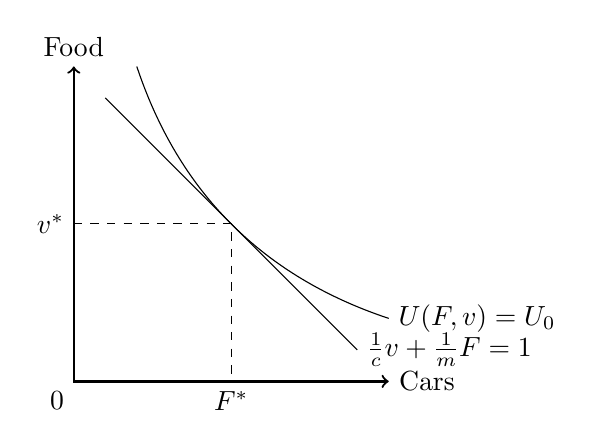
\begin{tikzpicture}[scale=0.4]

\draw[thick,<->] (0,10) node[above]{Food}--(0,0)--(10,0) node[right]{Cars};

\node [below left] at (0,0) {$0$};

\node [below] at (5,0) {$F^{*}$};

\node [left] at (0,5) {$v^{*}$};

\draw(1,9)--(9,1) node[right]{$\frac{1}{c} v + \frac{1}{m} F = 1$};

\draw[dashed](0,5)--(5,5)--(5,0);

\draw(2,10) ..controls (3.33,6) and (6,3.33) .. (10,2) node[right]{$U(F,v)=U_0$};

\end{tikzpicture}$$

However, this cannot pin down time usage. From the initial
constraints, it is known that the time spent working will be given by:
\begin{equation*}
  \ell = 1 - \frac{f_H}{m}
\end{equation*}
In equilibrium, the individual is indifferent between
producing and consuming food at home or the marketplace. It is
equivalent to think about the consumers spending all of his time
working, and then spending some of the money earned on food in the
marketplace as it is to believe that the consumer buys no food at the
marketplace, working only to buy cars.

There is a minimum time required to spend working. The consumer cannot
substitute car production in the household, so he must work to earn
the wages required to purchase the cars on the market. Let $v^{*}$ be the
optimal amount of cars used.
\begin{equation*}
  \ell_{min} = v^{*} \frac{p_v}{w} = \frac{v^{*}}{c}
\end{equation*}

This is the amount of time required to earn the money to buy the
optimal amount of cars. The consumer is indifferent between working
this amount and any amount above it, capped at one.

Note that the consumer's budget constraint could be rewritten as:
\begin{equation*}
  1 = \frac{1}{c} v + \frac{1}{m}F
\end{equation*}
That is, the prices faced by the consumer are equal to the time
required to produce a single unit of that item. Therefore as $m$ goes
up, individuals find producing food less costly, and believe that they
have relatively more time. If we believe that the ``income effect'' of
having what appears to be more time is dominated by the substitution
effect, then the individual will produce more food. The same logic
applies for an increase in $c$.

\section*{Part B}
It does not matter if meals are produced in the market or at home. In
equilibrium, the cost of substituting between making food at home and
buying the food is the same to the consumer, and the benefit is
clearly the same. As long as food consumption is positive, there
are an infinite number of equilibria where different amounts of time
are spent producing food in the firm and in the household.

\section*{Part C}

These taxes affect the revenues earned by each of the firms. Their
zero-profit conditions become: 
\begin{align*}
  .9 p_f m  = w_f = w \quad \quad & p_f = \frac{10 w}{9 m} \quad \quad   \frac{p_f}{p_v} = \frac{c}{m}
 \\
  .9 p_v c  = w_v = w \quad \quad &p_v = \frac{10 w}{9 c}\\
\end{align*}

We still have the same relationship for the relative prices as
before. Let us examine the new consumer's problem:

\begin{align*}
  \max_{v,f_m,f_H} \quad&U( f_H + f_m, v)\\
  \text{s.t} \quad& R + w\ell = p_v v + p_f f_m\\
  & \ell \in [0,1]
\end{align*}

Applying the equilibrium prices to our constraints:

\begin{align*}
  \max_{v,f_m,f_H} \quad&U( f_H + f_m, v)\\
  \text{s.t} \quad& 1  + \frac{R}{w} = \frac{10}{9c} v + \frac{10}{9m} f_m
                + \frac{1}{m} f_H\\
  & f_H \in [0,m]
\end{align*}

In terms of time, the price of the market goods is relatively more
expensive to the individual, and their income has been
raised. As Household production of food is relatively cheaper than market
production of food, all food consumption will take
place in the home. Individuals will only work to consume cars, and will
work $c  = \frac{10 w}{9} v^{*}$ hours.

The wage relative to the price of cars that the consumer faces is
lower, but their income is subsidized by the government paying them
some quantity of money. This amount cannot be normalized by the wage
amount because each individual is setting his workload
individually. As a result, producing food in the home is relatively
cheaper, as he still receives this tax load when he works less. Labor
is competitive, he has no power in controlling the total amount of
work, and thus his taxable income. 

$$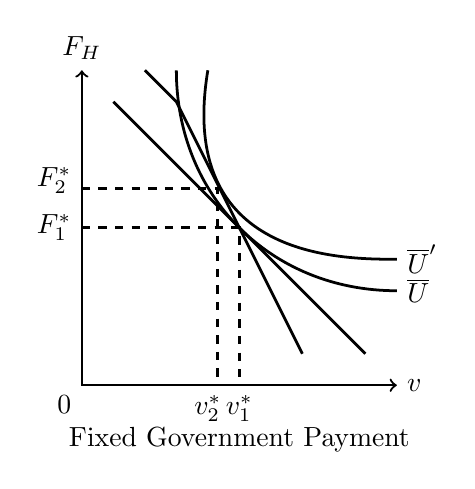
\begin{tikzpicture}[scale=0.4, line width = 1pt]

\draw[thick,<->] (0,10) node[above]{$F_H$}--(0,0)--(10,0) node[right]{$v$};

\node [below left] at (0,0) {$0$};

\node [below] at (4,0) {$v_2^{*}$};
\node [left] at (0,5) {$F_{1}^{*}$};
\node [below] at (5,0) {$v_1^{*}$};
\node [left] at (0,6.5) {$F_2^{*}$};

\node [below] at (5,-1){Fixed Government Payment};

\draw(1,9)--(9,1) node[right]{};
\draw(2,10)--(3,9)--(7,1) node[right]{};

\draw[dashed](0,5)--(5,5)--(5,0);
\draw[dashed](0,6.25)--(4.3,6.25)--(4.3,0);

\draw(3,10) ..controls (3,6) and (6,3) .. (10,3)
node[right]{$\overline{U}$};

\draw(4,10) ..controls (3,4) and (8.25,4) .. (10,4) node[right]{$\overline{U}^{\prime}$};

\end{tikzpicture}
\hspace{1cm}
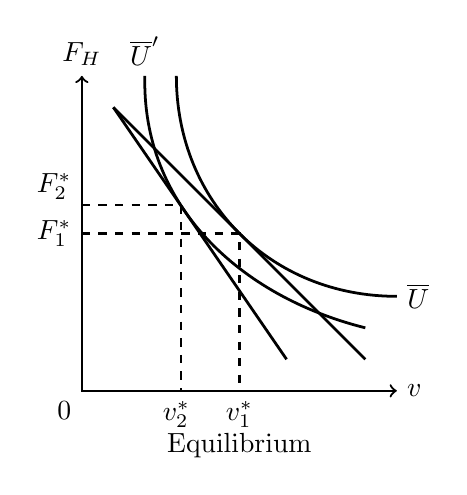
\begin{tikzpicture}[scale=0.4, line width = 1pt]

\draw[thick,<->] (0,10) node[above]{$F_H$}--(0,0)--(10,0) node[right]{$v$};

\node [below left] at (0,0) {$0$};

\node [below] at (3,0) {$v_2^{*}$};
\node [left] at (0,5) {$F_{1}^{*}$};
\node [below] at (5,0) {$v_1^{*}$};
\node [left] at (0,6.5) {$F_2^{*}$};

\draw(1,9)--(9,1) node[right]{};
\draw(1,9)--(6.5,1) node[right]{};

\draw[dashed](0,5)--(5,5)--(5,0);
\draw[dashed](0,5.9)--(3.15,5.9)--(3.15,0);

\draw(3,10) ..controls (3,6) and (6,3) .. (10,3)
node[right]{$\overline{U}$};

\draw(2,10) node[above]{$\overline{U}^{\prime}$} ..controls (1.9,5.9) and (5,3) .. (9,2);
\node [below] at (5,-1){Equilibrium};
\end{tikzpicture}$$


One important concept seen on this graph is that the original
consumption is always a choice for the worker. If he did not adjust
his behavior, his wage plus subsidy would allow him to purchase the
same bundle at market.  It will never be the case that he is worse off
under this tax. To face a higher utility, he must substitute food for
cars. This tells us that food consumption will rise and that car
consumption will fall. This will cause the government revenue to drop,
and the individuals receive less revenue from the government. Then
they must adjust their behavior accordingly. This process will
repeat.

They have less income than before, so their budget line lowers. If
they elected to work $0$ hours, they could produce the same amount of
food at home as pre-tax as the equilibrium government payout would be
$0$. Cars are relatively more expensive, so the slope of the budget
line is steeper. This gives us the equilibrium budget line on the graph
on the right. and the lower equilibrium utility level
$\overline{U}^{\prime}$. Consumers must work less, and therefore receive a
lower income because of the government than before the tax. This
limits their possible consumption of vehicles to less than it was
before the tax, causing an inward shift of their budget set. In
equilibrium they reach a lower level of utility than before the
tax. If we believe that cars are a normal good, consumers will strictly
consume less cars in the post-tax equilibrium. Food is relatively
cheaper, but income has decreased, so the change in food consumption
will be indeterminate. 


\section*{Part D}

Now the consumers face a cost of switching between working for the
firm that produces food and the firm that produces cars. The cost is
$k$ units of time that they must spend learning how the use the
machinery in order to begin working for the car-producing firm. Note
that if the consumer elects to face this fixed cost, he will spend all
of his working time working to produce cars. If he chooses not to, all
of his working time will be spent producing food. He earns a higher
wage working for car production, so there is no reason for him to
split his time and earn the lower wage after facing the fixed cost.

Since there is an extra cost to working at only one firm, we should
not expect the wages to be equal in equilibrium. The car firms will
provide a higher wage in order to attract workers to pay this cost of
time spent learning. Both firms however will continue to earn zero
profits in equilibrium.

\begin{align*}
  p_v c L_v - w_v L_v = 0 &\quad \quad p_f m L_f - w_f L_f = 0\\
  p_v c = w_v & \quad \quad p_f m = w_f
\end{align*}

In equilibrium, the consumer will be indifferent between working at
producing cars, and working at producing food. Otherwise all consumers
would work for one firm, and there would be no production of the other
good. This means that either choice of job should live on the same
indifference curve.

If the consumer were to work for the food producing firm, the question
is as before: But with the only choice of working is producing food
for the market. He does face a higher price in time for cars. This
occurs because $p_v c = w_v > w_f$ in our equilibrium. The mechanism
of his choice remains the same, and he will still maximize utility as
if he were facing two goods: food and cars each with a price
determined by the market. The shadow price of making food at home
remains equal to the market price of food.

If the consumer elects to work in car-production, his utility
maximization problem is as follows:

\begin{align*}
\max_{f_H,f_m,v,\ell} \quad &U( f_H + f_m)\\
  \text{s.t.} \quad & w_v \ell = p_f f_{m} + p_v v\\
                & (1 - \ell - k)m = f_H\\
                & \ell \in [0,1-k]
\end{align*}

The second constraint can be rewritten as:
$\ell = 1 - \frac{f_H}{m} - k$. Applying this to the first constraint
gives us:

\begin{align*}
  (1-k)w_v = p_f f_m + p_v v + \frac{w_v}{m} f_H \\
  (1-k)w_v = \frac{w_f}{m} f_m + \frac{w_v}{c} v + \frac{w_v}{m} f_H\\
  (1-k) = \frac{w_f}{w_v} \frac{1}{m}  f_m + \frac{1}{c} v + \frac{1}{m} f_H
\end{align*}

Contrast this to the budget curve faced by the consumer who works for
the food firms.
\begin{align*}
  w_f = p_f f_m + p_v v + \frac{w_f}{m} f_H\\
  w_f = \frac{w_f}{m} f_m + \frac{w_v}{c} v + \frac{w_f}{m} f_H\\
  1 = \frac{1}{m} f_m + \frac{w_v}{w_f} \frac{1}{c} v + \frac{1}{m} f_H
\end{align*}


As the wages offered to the workers in the car workers are higher,
$\frac{w_f}{w_v} < 1$ and the price of food in the market is less than
the shadow price of producing food in the home. Car workers will
no longer be indifferent between producing food at home and in the
market, and will buy all of their food at market. This also implies
that they will spend all of their time working i.e. $\ell = 1 - k$.

When we assume that cars and meals are consumed in fixed proportions,
we assume the goods are perfect complements. Let $\alpha$ be the proportion
of food that consumers buy relative to the number of cars. One
important property of the Leontief is that the only place where a cost
minimizing consumers will choose to be is the vertex of the
indifference curve.

Note that consumers must be indifferent between working for either the
car or food firms. Since the only optimal consumption bundle on an
indifference curve is the vertex, both types of consumers must have
the same consumption bundles. Food working consumers are indifferent
between working and buying their food, and producing the food at
home. For the sake of the plot, assume that they choose to buy all
their food at the market. They face the same prices in the market, so
for the same consumption they must have equal income. This means that
either consumer faces the same budget constraint.  This implies
$w_v (1-k) = w_f$.

$$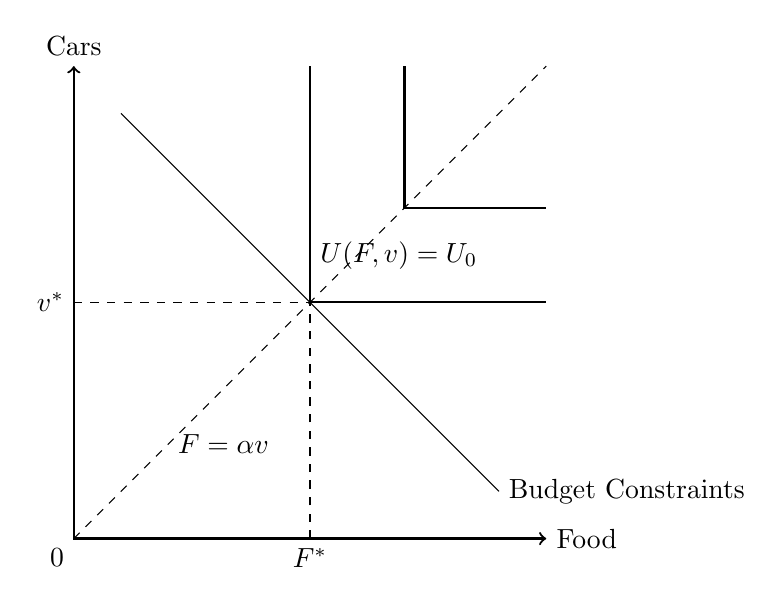
\begin{tikzpicture}[scale=0.6]

\draw[thick,<->] (0,10) node[above]{Cars}--(0,0)--(10,0) node[right]{Food};

\node [below left] at (0,0) {$0$};

\draw[dashed] (0,5)--(5,5);
\draw[dashed] (5,0)--(5,5);
\node [below] at (5,0) {$F^{*}$};
\node [left] at (0,5) {$v^{*}$};

\draw(1,9)--(9,1) node[right]{Budget Constraints};
\draw[thick](5,10)--(5,6)node[right]{$U(F,v)=U_0$}--(5,5)--(10,5);
\draw[thick](7,10)--(7,8)node[right]{}--(7,7)--(10,7);

\draw[dashed](0,0)--(2,2)node[right]{$F = \alpha v$}--(10,10);

\end{tikzpicture}$$

This will be governed by the following system:
\begin{align*}
  (1-k) &= \frac{w_v}{w_f m} f_m + \frac{1}{c} v\\
  \frac{w_v}{w_f} &= 1-k\\
  f_m &= \alpha v
\end{align*}

Note that $k, m, c, \alpha$ are fixed in this scenario, and
$f_m,v, \frac{w_f}{w_v}$ are three unknowns in a system of three
equations. As long as this system is consistent, it will determine the
consumption and relative wages.

Clearly everyone will work, as their utility with no consumption of
cars is zero due to the Leontief utility function. Cars cannot be
produced at home so these must be bought with wages. Therefore all
types of workers will choose to work, and the ones that work producing
cars will spend all of their available time working, and then purchase
food in the market.

The consumers that produce food will surely work some minimum amount, which
earns them enough wages to pay for their consumption of cars. They are
indifferent between working more and using this wage to buy food at
the market, and producing the food at home, so nothing can be said
about the exact amount that they choose to work.

\section*{Part E}
Solving this system of equations, we arrive at:
\begin{align*}
  \frac{w_v}{w_f} &= (1-k)\\
  v &= \frac{m c (1-k)}{(1-k)\alpha c + m}\\
  f_m &= \frac{c m \alpha (1-k)}{(1-k) \alpha c + m}
\end{align*}

Immediately we can see that $k$ has no effect on the amount of
consumption of the consumers, and can only affect the relative
wages of the two types of consumers. As $k \downarrow 0$, we can see that the
relative wage converges to $1$. This takes us to the scenario solved
in part A.

\begin{equation*}
  \frac{\partial \frac{w_v}{w_f}}{\partial k} = -1 
\end{equation*}

This tells us that the magnitude of a change in $k$ has on the
relative wage is equal to the change in $k$. This occurs from the
Leontief utility function enforcing that both consumers face the same
budget constraint.

The relative wage is proportional to the relative prices for the
consumer:
\begin{equation*}
  \frac{p_v}{p_f} = \frac{w_v m }{w_f c} = (1-k) \frac{m}{c}  
\end{equation*}

As $k$ rises, the relative prices of cars fall, scaled by the
technology. The larger the fixed cost, the less expensive cars are
relative to food. 

\section*{Part F}
The above analysis is independent of the magnitude of $k$ so
its result apply for both a small and a large value of $k$.

For any $k \in (0,1)$ we will find that all consumers will work. The
consumer will have some portion of free time, call it $\epsilon$. This time
can be spent working to earn $w_v \epsilon$, and this can be used to buy some
amount of food and cars. Due to the Leontief utility function,
consuming the small amount is strictly better than consuming nothing.

The consumers that work for the car firm will continue to work their
entire time, and buy food from the market as it is cheaper than
producing the food at home. The consumers working for the food firms
are still indifferent between buying their food at the market and
making the food at home. Some food at least will always be produced
and sold at market since there is a known demand for food, by the
workers who build cars, and supplied by the food workers using this
money to buy cars. There could be more demand and supply where the
workers produce food at the firm and consume that amount spending
their entire wage, but this will still be in equilibrium. As such, we
do not know how much work the food workers will choose to do. We do
know that the car workers will spend all of their available time
$(1-k)$ to produce cars. There is still a minimum amount of work that
the food producers will work, which is enough work to earn the wages
to buy the amount of cars they choose to produce.




\end{document}
